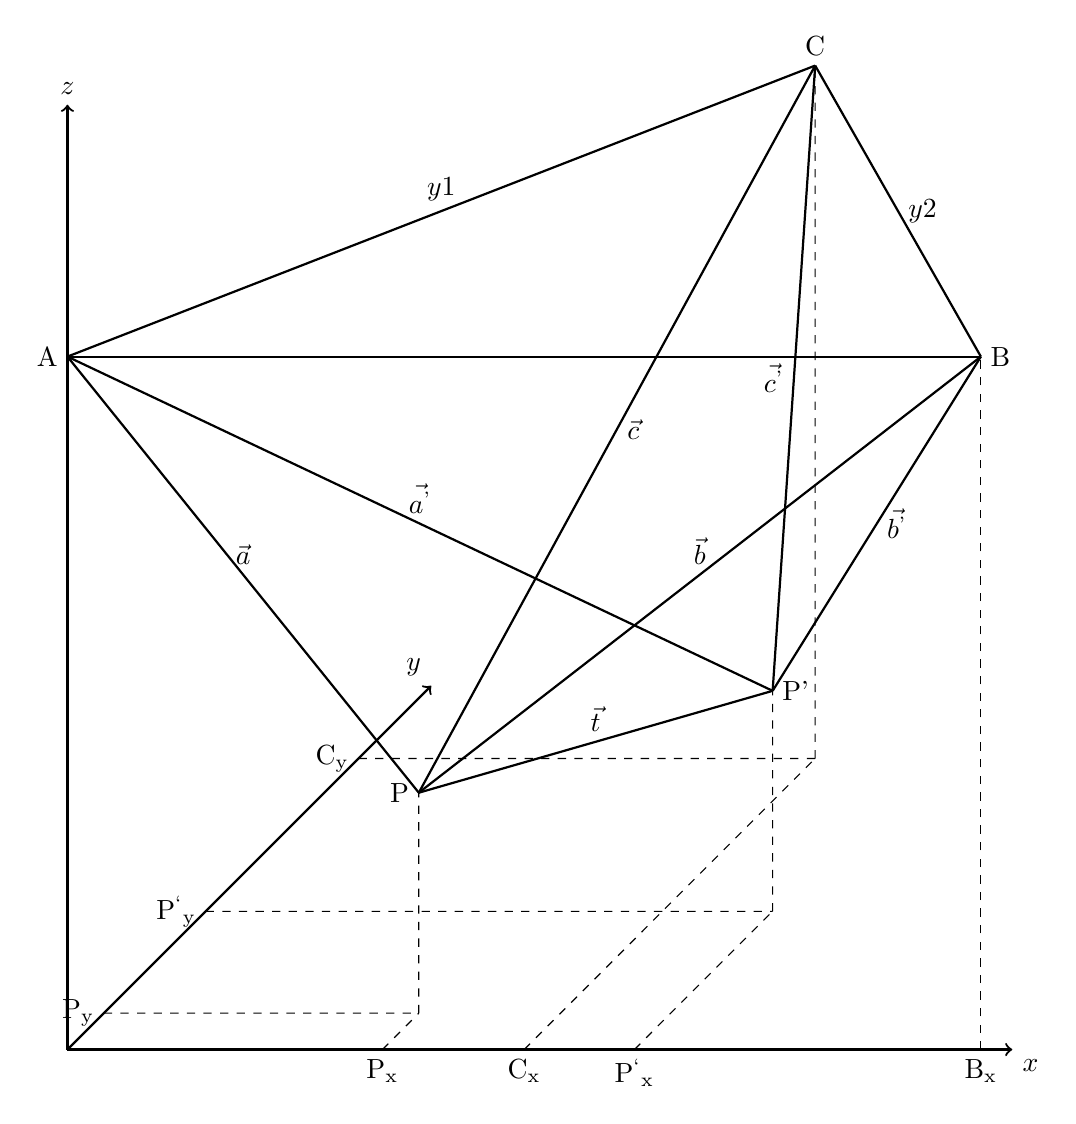
\begin{tikzpicture}[scale=0.8]
\coordinate 	[label=left:A] 										(A) 	at 	(0,11,0);
\coordinate 	[label=right:B] 									(B) 	at 	(14.5,11,0);
\coordinate 	[label=above:C] 									(C) 	at 	(7.25,11,-12);
\coordinate 	[label=left:P] 										(P) 	at 	(5,3.5,-1.5);
\coordinate 	[label=right:P'] 									(P') 	at 	(9,3.5,-5.7);

\coordinate		[label=left:P\textsubscript{y}]						(YP)	at 	(0,0,-1.5);
\coordinate		[label=below:P\textsubscript{x}]					(XP)	at 	(5,0,0);
\coordinate		[label=left:P\textsuperscript{`}\textsubscript{y}]	(YP')	at 	(0,0,-5.7);
\coordinate		[label=below:P\textsuperscript{`}\textsubscript{x}]	(XP')	at 	(9,0,0);
\coordinate		[label=below:B\textsubscript{x}]					(XB)	at 	(14.5,0,0);
\coordinate		[label=below:C\textsubscript{x}]					(XC)	at 	(7.25,0,0);
\coordinate		[label=left:C\textsubscript{y}]					    (YC)	at 	(0,0,-12);

%(x		,z		,y)
\draw[thick,->] (0,0,0) 		-- 	(15,0,0) 		node[anchor=north west]	{$x$};
\draw[thick,->] (0,0,0) 		-- 	(0,0,-15) 		node[anchor=south east]	{$y$};
\draw[thick,->] (0,0,0) 		-- 	(0,15,0) 		node[anchor=south]		{$z$};	
\draw[thick] 	(A) 			-- 	(B) 			;		
\draw[thick] 	(B) 			-- 	(C) 			node[midway,right]{$y2$};	
\draw[thick] 	(C) 			-- 	(A) 			node[midway,above]{$y1$};	
\draw[thick] 	(A) 			-- 	(P) 			node[midway,above]{$\vec{a}$};
\draw[thick] 	(A) 			-- 	(P') 			node[midway,above]{$\vec{a\textsuperscript{'}}$};
\draw[thick] 	(B) 			-- 	(P) 			node[midway,above]{$\vec{b}$};
\draw[thick] 	(B) 			-- 	(P') 			node[midway,right]{$\vec{b\textsuperscript{'}}$};
\draw[thick] 	(C) 			-- 	(P) 			node[midway,right]{$\vec{c}$};
\draw[thick] 	(C) 			-- 	(P') 			node[midway,left] {$\vec{c\textsuperscript{'}}$};
\draw[thick] 	(P) 			-- 	(P') 			node[midway,above]{$\vec{t}$};
\draw[dashed,-]  (XB) 			-- 	(B) 		;
\draw[dashed,-]  (XC) 			-- 	(7.25,0,-12) 		;
\draw[dashed,-]  (YC) 			-- 	(7.25,0,-12) 		;
\draw[dashed,-]  (7.25,0,-12) 	-- 	(C) 		;
\draw[dashed,-]  (XP) 			-- 	(5,0,-1.5) 		;
\draw[dashed,-]  (YP) 			-- 	(5,0,-1.5) 		;
\draw[dashed,-]  (5,0,-1.5) 	-- 	(P);
\draw[dashed,-]  (XP') 			-- 	(9,0,-5.7) 		;
\draw[dashed,-]  (YP') 			-- 	(9,0,-5.7) 		;
\draw[dashed,-]  (9,0,-5.7) 	-- 	(P');
\end{tikzpicture}
\caption{Darstellung der Transformation eines Punktes im Zweidimensionalen}
				